\chapter*{\centering{Appendices}}
 \appendix
 \pagenumbering{roman}
 \chapter{Stewart Platform and Wind Tunnel Configurations}
 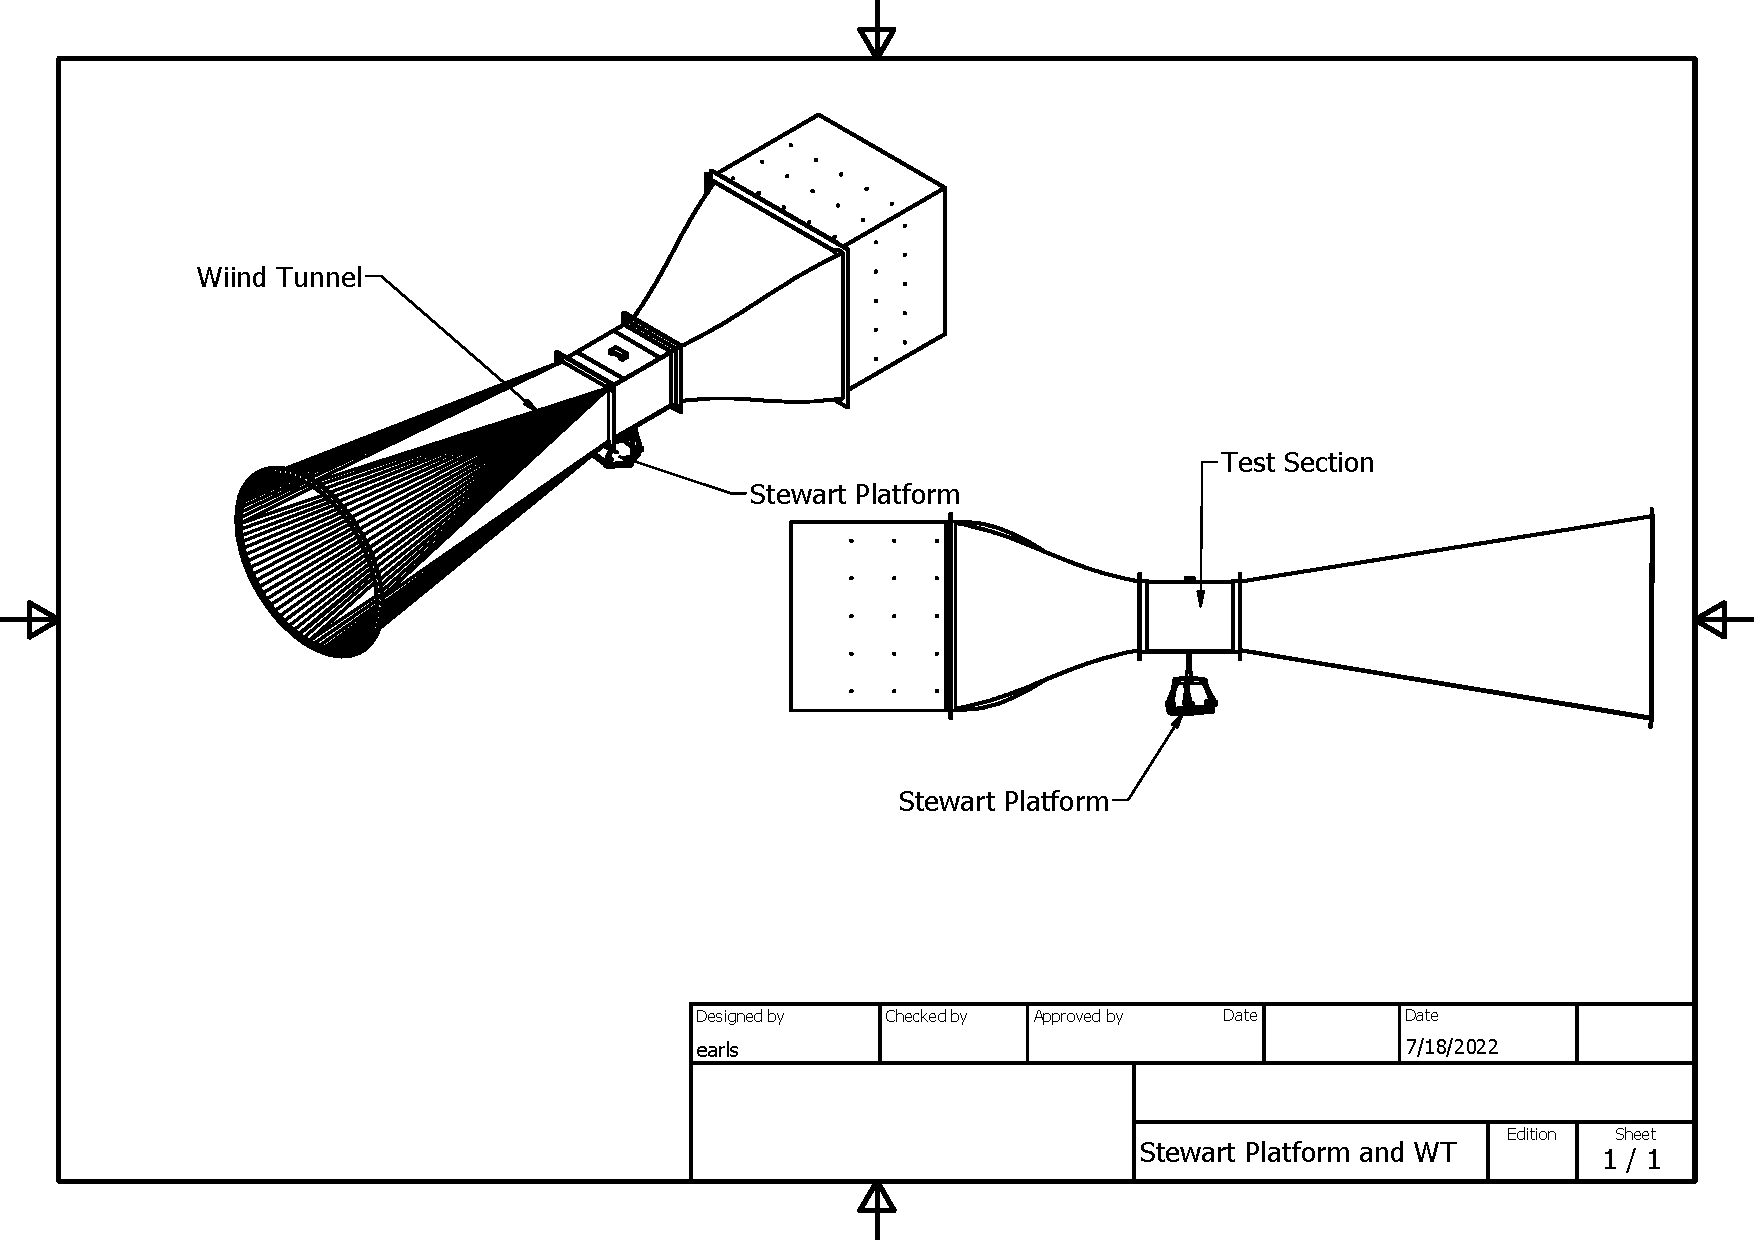
\includepdf[pages=-]{Wind Tunnel Assembly + Stewart}
 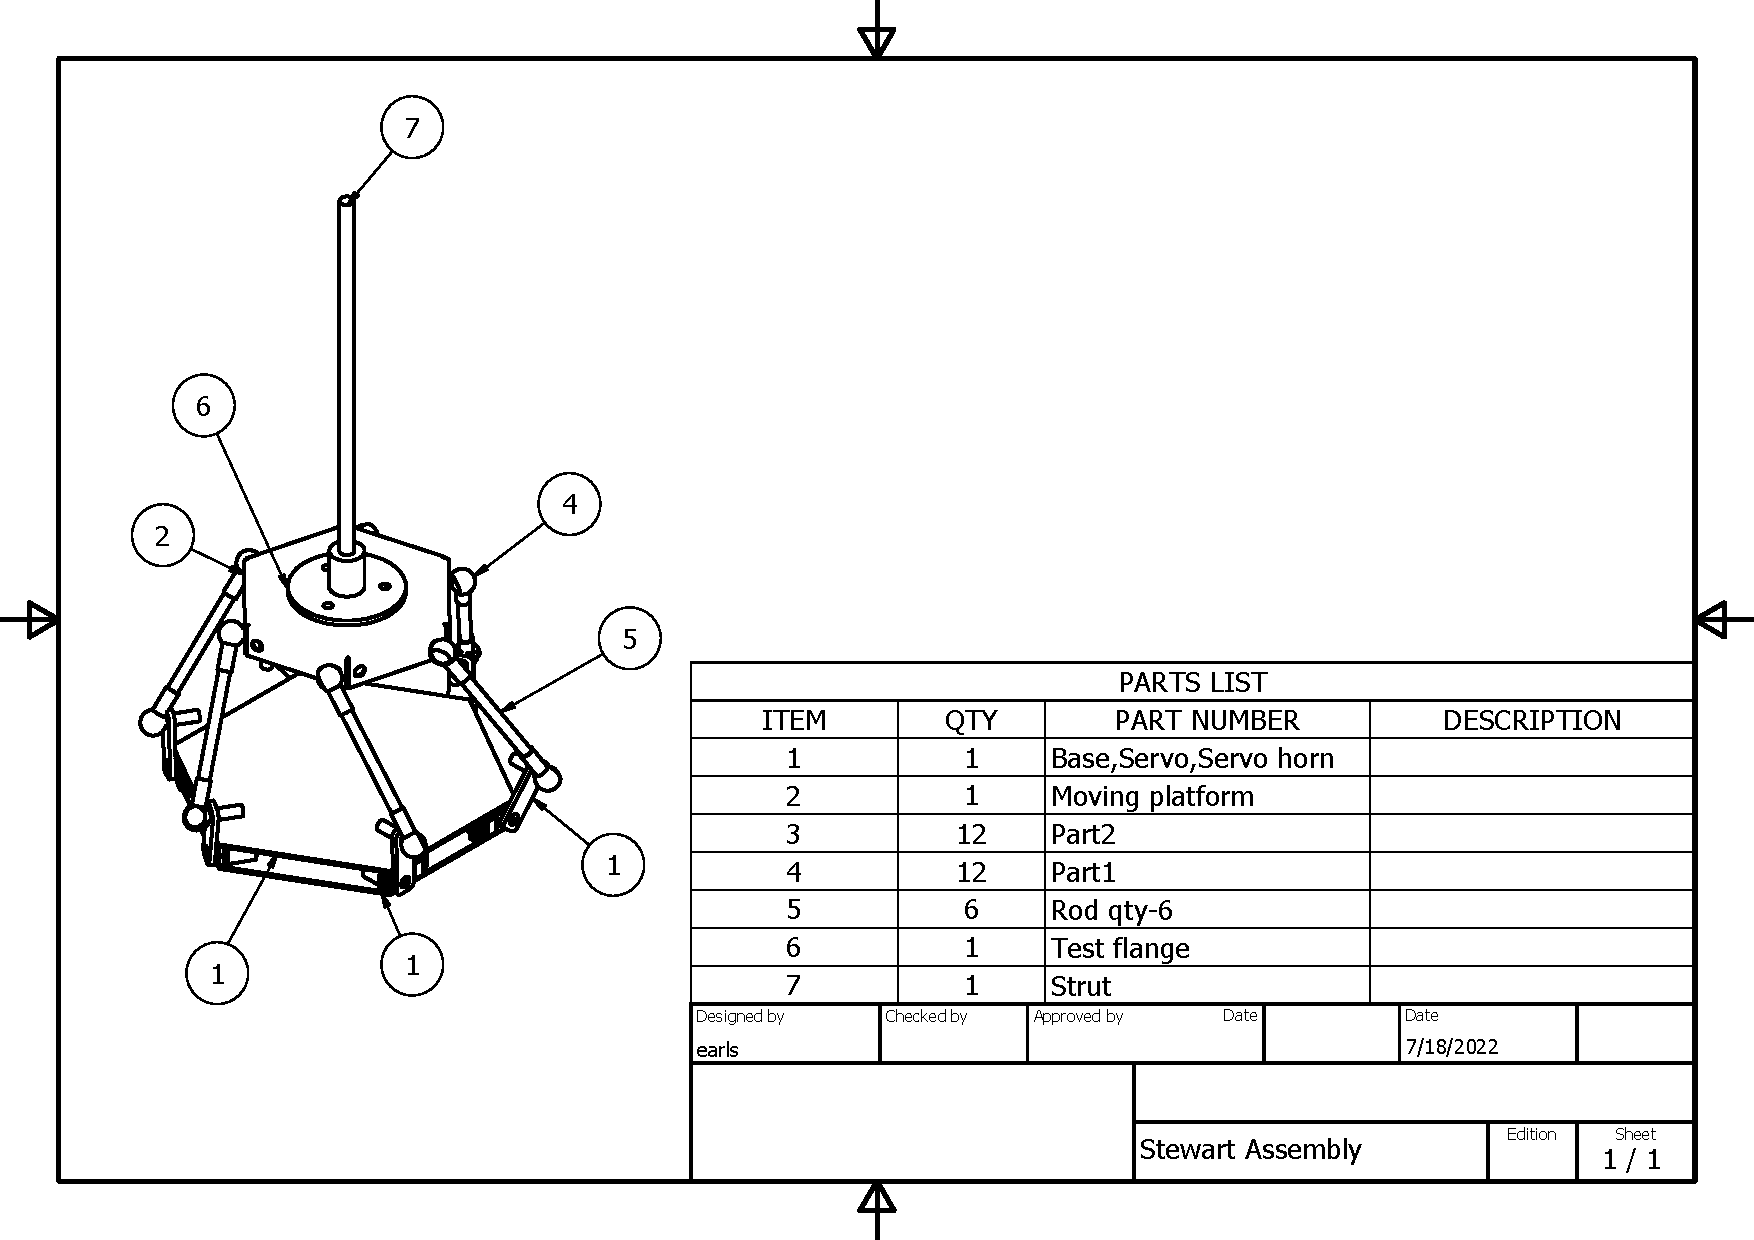
\includepdf[pages=-]{Assemby 3 2}
 \chapter{Budget and Timeplan}
 \section{Provisional Budget}
 \begin{center}
 \begin{table}[!h]
 \centering
 \caption{Proposed budget}
 \paragraph{ }
 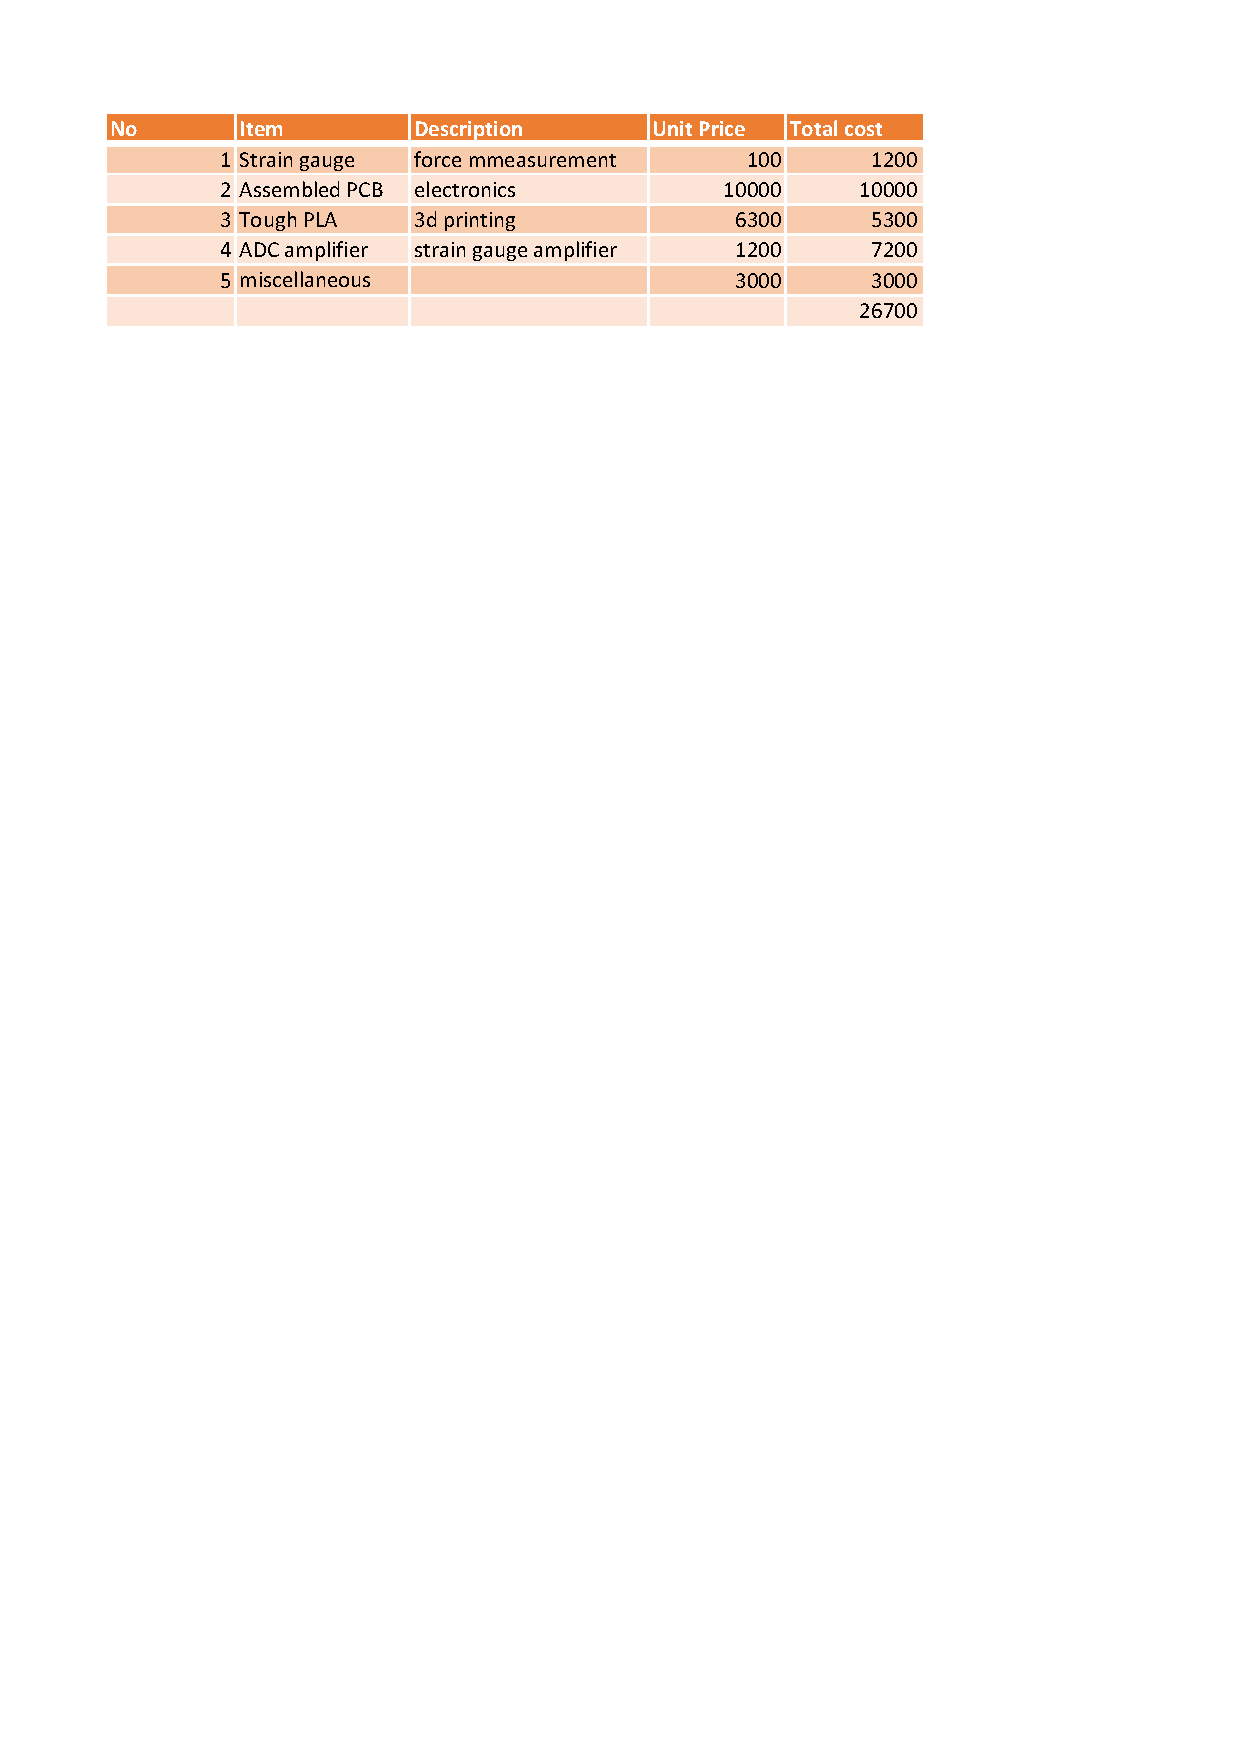
\includegraphics{Figures/budget}
 \end{table}
 \end{center}
 \section{Work Plan}
 \begin{center}
 \begin{table}[!h]
 \centering
 \caption[Timeplan]{Timeplan for first and second semester}
 \paragraph{ }
 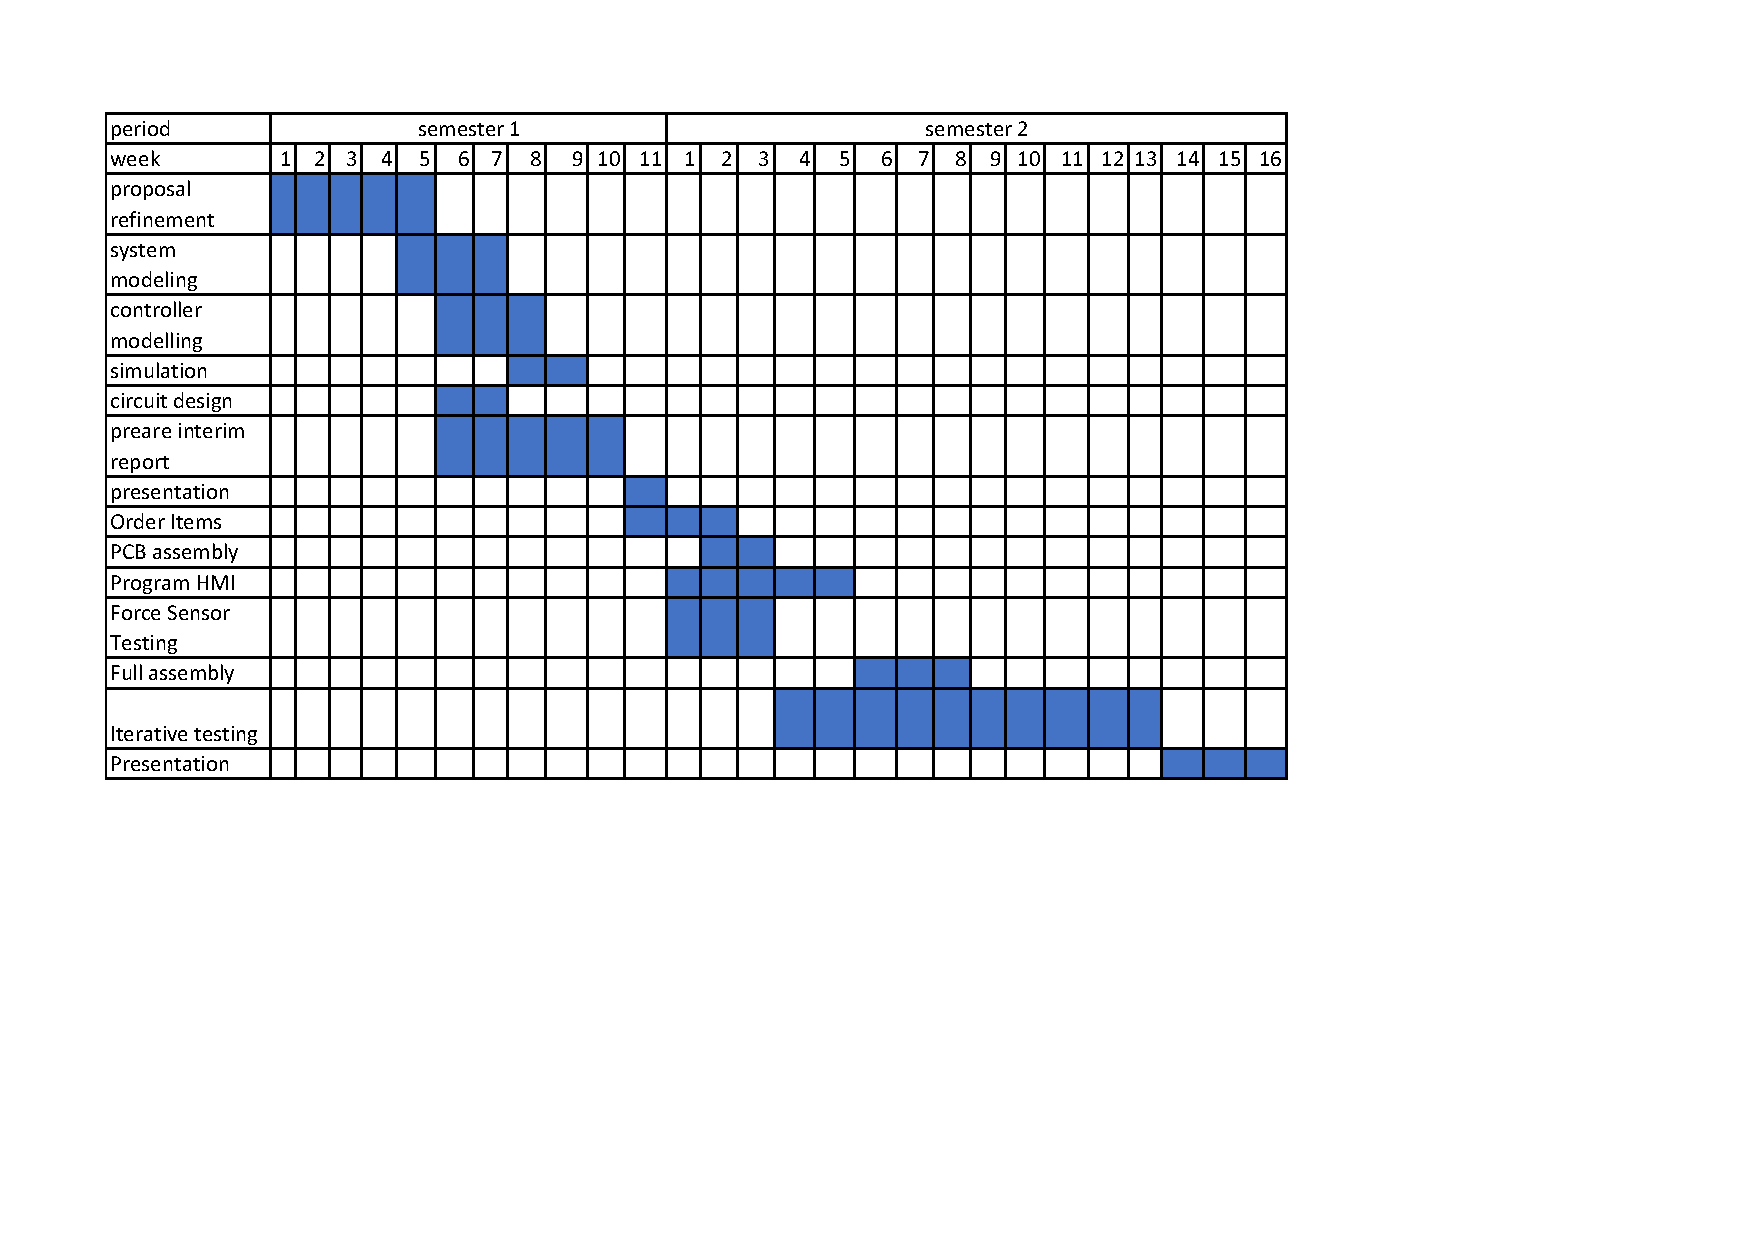
\includegraphics[width=0.95\linewidth]{Figures/workplan}
 \end{table}
 \end{center}
\chapter{HMI code}
 \section{Program}
 \begin{verbatim}
 package main
 
 import (
 	"fyne.io/fyne/v2"
 	"fyne.io/fyne/v2/app"
 	"fyne.io/fyne/v2/container"
 	"fyne.io/fyne/v2/data/binding"
 	"fyne.io/fyne/v2/layout"
 	"fyne.io/fyne/v2/widget"
 )
 
 func main() {
 	a := app.New()
 	w := a.NewWindow("Force Balance")
 
 	dashHome := widget.NewLabel("Stewart Platform Force-Balance Dashboard!")
 	fYaw := 0.0
 	fRoll := 0.0
 	fPitch := 0.0
 	xtrans := 0.0
 	ytrans := 0.0
 	ztrans := 0.0
 
 	yawLabel, yawSlider := getNewSliderWithLabel(&fYaw, -5.0, 5.0)
 	rollLabel, rollSlider := getNewSliderWithLabel(&fRoll, -5.0, 5.0)
 	pitchLabel, pitchSlider := getNewSliderWithLabel(&fPitch, -5.0, 5.0)
 	xtransLabel, xtransSlider := getNewSliderWithLabel(&xtrans, -4.0, 4.0)
 	ytransLabel, ytransSlider := getNewSliderWithLabel(&ytrans, -4.0, 4.0)
 	ztransLabel, ztransSlider := getNewSliderWithLabel(&ztrans, -4.0, 4.0)
 
 	sliderLayout := layout.NewAdaptiveGridLayout(2)
 
 	yprBox := container.NewVBox(
 		widget.NewLabel("Yaw"),
 		yawLabel,
 		yawSlider,
 		widget.NewLabel("Pitch"),
 		pitchLabel,
 		pitchSlider,
 		widget.NewLabel("Roll"),
 		rollLabel,
 		rollSlider,
 	)
 	xyzBox := container.NewVBox(
 		widget.NewLabel("x"),
 		xtransLabel,
 		xtransSlider,
 		widget.NewLabel("y"),
 		ytransLabel,
 		ytransSlider,
 		widget.NewLabel("z"),
 		ztransLabel,
 		ztransSlider,
 	)
 
 	w.SetContent(container.NewVBox(
 		dashHome,
 		fyne.NewContainerWithLayout(
 			sliderLayout,
 			yprBox,
 			xyzBox,
 		),
 		fyne.NewContainerWithLayout(
 			sliderLayout,
 			widget.NewButton("Write Position", func() {}),
 			widget.NewButton("Record Data", func() {}),
 		),
 	))
 
 	w.ShowAndRun()
 }
 
 func getNewSliderWithLabel(num *float64, min float64, max float64) (*widget.Label, *widget.Slider) {
 	data := binding.BindFloat(num)
 	yprSilder := widget.NewSliderWithData(min, max, data)
 	label := widget.NewLabelWithData(
 		binding.FloatToString(data),
 	)
 	return label, yprSilder
 }
 
 \end{verbatim}
 
 \chapter{PCB schematics}
 \section{schematics}
 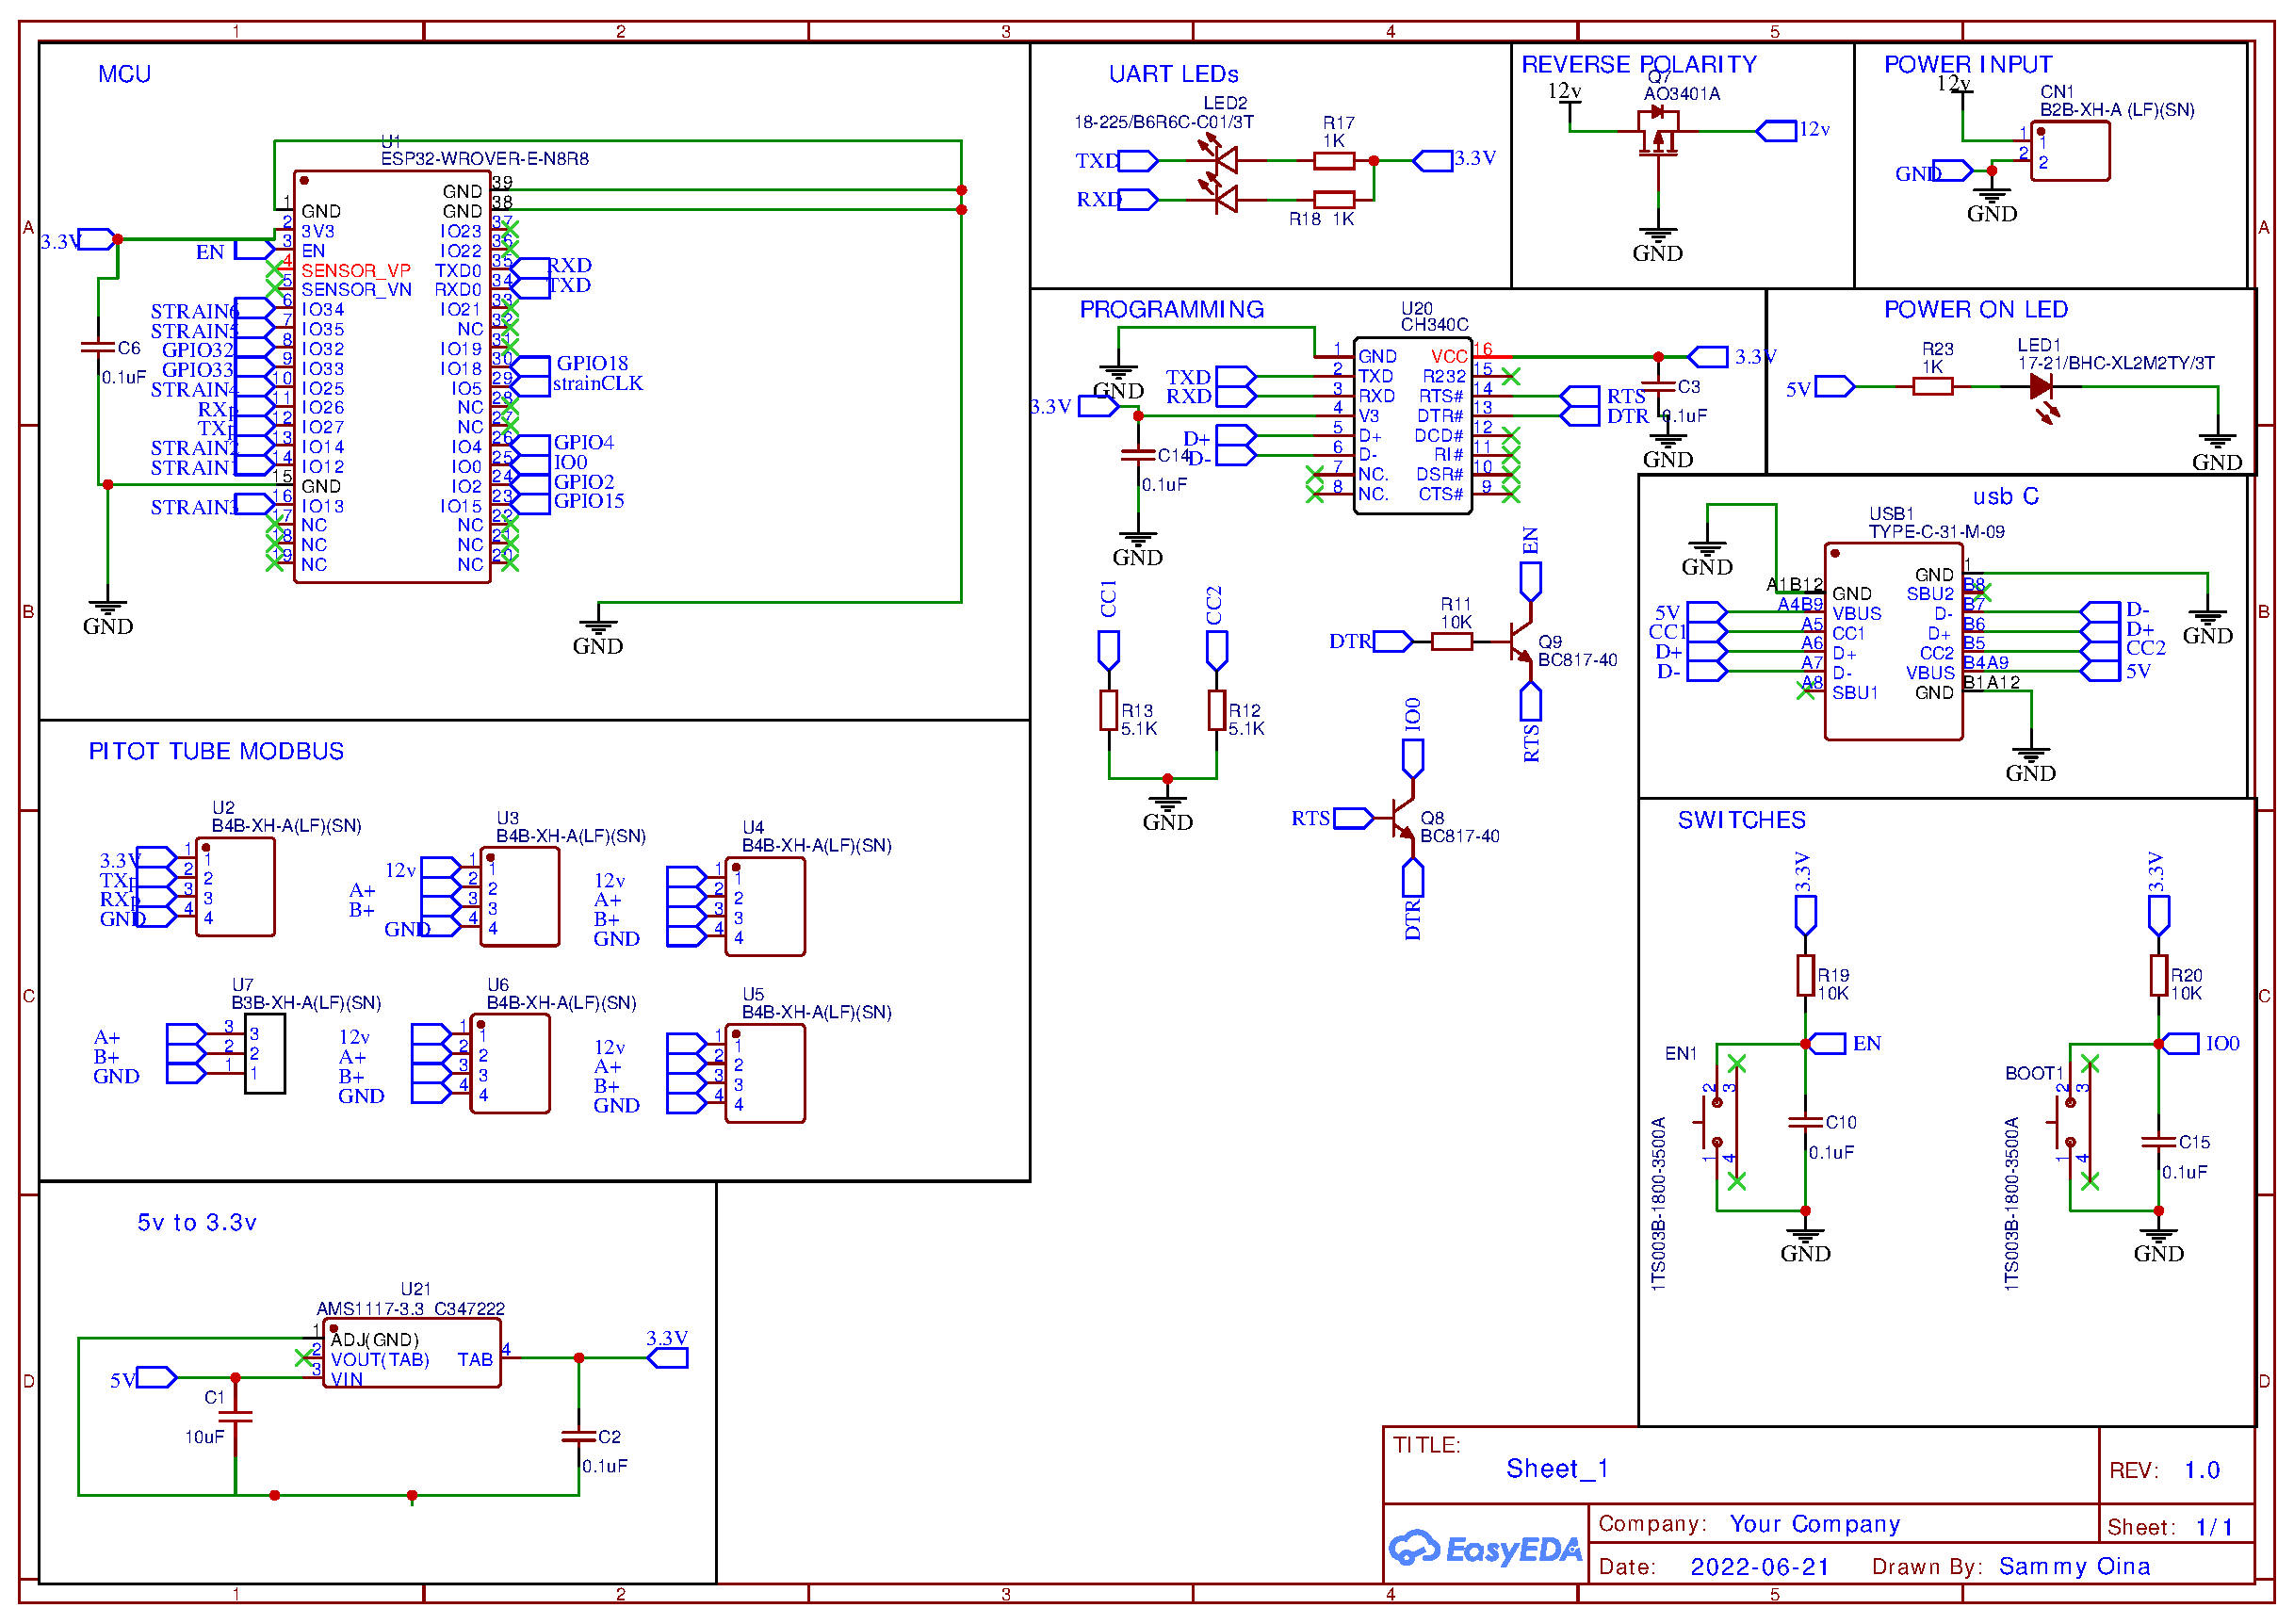
\includepdf[pages=-]{Figures/schm}